\onehalfspacing
\section{Đề số 29}

\begin{bt} 
   \hfill
   \begin{enumerate}[a.]
    \item  Tìm $x$, biết $|x-1|=\frac{2}{3}$;
    \item Tính giá trị của biểu thức sau: $\mathrm{A}=\frac{2 \mathrm{x}^2+3 x-1}{3 x-2}$ với $|x-1|=\frac{2}{3}$
   \end{enumerate}
\loigiai{
    \begin{enumerate}
        \item Ta có $|x-1|=\frac{2}{3} \Leftrightarrow\left[\begin{array}{c}x-1=\frac{2}{3} \\[5px] x-1=-\frac{2}{3}\end{array} \Leftrightarrow\left[\begin{array}{l}x=\frac{5}{3} \\[5px] x=\frac{1}{3}\end{array}\right.\right.$
        \item Từ câu 1):\\[5px] 
        Với $\mathrm{x}=\frac{5}{3}$ thay vào $\mathrm{A}$ ta được $\mathrm{A}=\frac{14}{27}$\\[5px] 
        Với $x=\frac{1}{3}$ thay vào $\mathrm{A}$ ta được $\mathrm{A}=-\frac{2}{9}$
    \end{enumerate}
}
\end{bt}

\begin{bt}
    \hfill
	\begin{enumerate}[a.]
        \item Tìm chữ số tận cùng của $A$ biết $A=3^{n+2}-2^{n+2}+3^n-2^n$
        \item Tìm các giá trị nguyên của $x$ để $\frac{x+3}{x-2}$ nhận giá trị nguyên.
    \end{enumerate}
	\loigiai{
        \begin{enumerate}
            \item Ta có:\\[5px]
            $A =3^{n+2}-2^{n+2}+3^n-2^n=3^n\left(3^2+1\right)-2^n\left(2^2+1\right)=10.3^n-2^n\left(2^2+1\right)=10.3^n-5.2^n \\[5px]
            =10.3^n-10.2^{n-1}=10\left(3^n-2^{n-1}\right) \vdots 10$\\[5px]
            A chia hết cho 10 suy ra chữ số tận cùng của $A$ là 0
            \item Ta có:\\[5px]
            $\frac{x+3}{x-2}=\frac{x-2+5}{x-2}=1+\frac{5}{x-2} \in Z \Leftrightarrow x-2 \in U(5)=\{ \pm 1 ; \pm 5\} \\[5px]
            \Rightarrow x=1 ; 3 ;-3 ; 7$
        \end{enumerate}
    } 
\end{bt}

\begin{bt}
    Cho đa thức $f(x)$ xác định với mọi $x$ thỏa mãn: $x \cdot f(x+2)=\left(x^2-9\right) \cdot f(x)$.
    \begin{enumerate}[a.]
        \item Tính $f(5)$.
        \item Chứng minh rằng $\mathrm{f}(\mathrm{x})$ có ít nhất 3 nghiệm.
    \end{enumerate}
	\loigiai{
        \begin{enumerate}
            \item Ta có với $x=3 \Rightarrow f(5)=0$
            \item $x=0 \Rightarrow f(0)=0 \Rightarrow x=0$ là một nghiệm\\[5px] 
            $x=3 \Rightarrow f(5)=0 \Rightarrow x=5$ là một nghiệm\\[5px] 
            $x=-3 \Rightarrow f(-1)=0 \Rightarrow x=-1$ là một nghiệm\\[5px] 
            Vậy $\mathrm{f}(\mathrm{x})$ có ít nhất là 3 nghiệm.
        \end{enumerate}
    }
\end{bt}

\begin{bt}
    Cho tam giác $\mathrm{ABC}$, trung tuyến $\mathrm{AM}$. Trên nửa mặt phẳng chứa đỉnh $\mathrm{C}$ bờ là đường thẳng $\mathrm{AB}$ dựng đoạn $\mathrm{AE}$ vuông góc với $\mathrm{AB}$ và $\mathrm{AE}=\mathrm{AB}$. Trên nửa mặt phẳng chứa đỉnh $\mathrm{B}$ bờ là đường thẳng $\mathrm{AC}$ dựng đoạn $\mathrm{AF}$ vuông góc với $\mathrm{AC}$ và $\mathrm{AF}=\mathrm{AC}$. Chứng minh rằng:
    \begin{enumerate}[a.]
        \item $F B=E C$
        \item $\mathrm{EF}=2 \mathrm{AM}$
        \item $\mathrm{AM} \perp \mathrm{EF}$.
    \end{enumerate}
	\loigiai{
        $$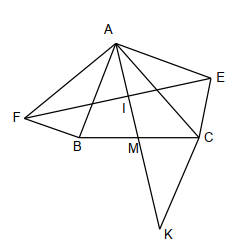
\includegraphics[width=0.45\textwidth]{29-4-lg.png}$$
        \begin{enumerate}
            \item Chứng minh $\triangle A B F=\triangle A E C(\operatorname{cgc}) \Rightarrow F B=E C$
            \item Trên tia đối của tia MA lấy $\mathrm{K}$ sao cho $\mathrm{AK}=2 \mathrm{AM}$. Ta có:\\[5px]
            $\triangle \mathrm{ABM}=\Delta \mathrm{KCM} \Rightarrow \mathrm{CK} / / \mathrm{AB} \\[5px]
            \Rightarrow A C K+C A B=E A F+C A B=180^{\circ} \Rightarrow A C K=E A F \\[5px]
            \triangle \mathrm{EAF} \text { và } \triangle \mathrm{KCA} \text { có } \mathrm{AE}=\mathrm{AB}=\mathrm{CK} \text {; } \\[5px]
            \mathrm{AF}=\mathrm{AC}(\mathrm{gt}) ; A C K=E A F \\[5px]
            \Rightarrow \Delta \mathrm{EAF}=\Delta \mathrm{KCA}(\mathrm{cgc}) \Rightarrow \mathrm{EF}=\mathrm{AK}=2 \mathrm{AM} .$ \\[5px]
            \item Từ $\triangle \mathrm{EAF}=\Delta \mathrm{KCA} \Rightarrow C A K=A F E\\[5px] 
            \Rightarrow A F E+F A K=C A K+F A K=90^{\circ}$\\[5px] 
            $\Rightarrow A K \perp E F$
        \end{enumerate}
    }
\end{bt}

\begin{bt}
    Cho $a, b, c, d$ là các số dương. Tìm giá trị nhỏ nhất của biểu thức:
    $$
    A=|x-a|+|x-b|+|x-c|+|x-d|
    $$
\loigiai{
    Không mất tính tổng quát, giả sử $\mathrm{a} \leq \mathrm{b} \leq \mathrm{c} \leq \mathrm{d}$. Áp dụng BĐT $|a|+|b| \geq|a+b|$, dấu bằng xảy $\mathrm{ra} \Leftrightarrow \mathrm{ab} \geq 0$ ta có:\\[5px]
    $|x-a|+|x-d| \geq|x-a|+|d-x| \geq|x-a+d-x|=d-a \\[5px]
    |x-b|+|x-c| \geq|x-b|+|c-x| \geq|x-b+c-x|=c-b$\\[5px]
    Suy ra $\mathrm{A} \geq \mathrm{c}+\mathrm{d}-\mathrm{a}-\mathrm{b}$. Dấu "=" xảy ra khi và chỉ khi dấu "=" ở (1) và (2) xảy ra \\[5px] 
    $\Leftrightarrow(x-a)(d-x) \geq 0$ và $(x-b)(c-x) \geq 0 \Leftrightarrow \mathrm{a} \leq \mathrm{x} \leq \mathrm{d}$ và $\mathrm{b} \leq \mathrm{x} \leq \mathrm{c}$.\\[5px]
    Do đó $\min \mathrm{A}=\mathrm{c}+\mathrm{d}-\mathrm{a}-\mathrm{b} \Leftrightarrow \mathrm{b} \leq \mathrm{x} \leq \mathrm{c}$.
}
\end{bt}


